\documentclass{article}

% Language setting
% Replace `english' with e.g. `spanish' to change the document language
\usepackage[english]{babel}

% Set page size and margins
% Replace `letterpaper' with `a4paper' for UK/EU standard size
\usepackage[letterpaper,top=2cm,bottom=2cm,left=1cm,right=1cm,marginparwidth=1.75cm]{geometry}
\usepackage{matlab-prettifier}
% Useful packages
\usepackage{amsmath}
\usepackage{amssymb}
\usepackage{graphicx}
\usepackage{mathtools}
\usepackage{enumitem}
\usepackage[colorlinks=true, allcolors=blue]{hyperref}

\title{Approssimazione del minimo taglio normalizzato}
\author{Tommaso Dossi}
\newcommand{\W}{\mathbf{W}}
\newcommand{\D}{\mathbf{D}}

\begin{document}
\maketitle

%\begin{abstract}
%Your abstract.
%\end{abstract}

\section{Taglio Normalizzato}

Dato un grafo $G = (V,E)$ e una partizione di $V$ in due insiemi disgiunti $A$ e $B$,
il taglio normalizzato $Ncut(A,B)$ \`e una misura della bont\`a della partizione
al fine di suddividere il grafo in pi\`u componenti.
Pi\`u formalmente, sia:
\begin{equation*}
    assoc(X,Y) \coloneq \sum_{x \in X, y \in Y} w(x,y)
\end{equation*}

Il taglio normalizzato \`e definito come segue:
\begin{equation}
    Ncut(A,B) \coloneq \frac{assoc(A,B)}{assoc(A,V)} + \frac{assoc(A,B)}{assoc(B,V)}
\end{equation}

Questo differisce dalla classica definizione di taglio, ossia $assoc(A,B)$, poich\`e penalizza, ad esempio,
le partizioni dove $A$ \`e un nodo isolato.
A differenza del taglio non normalizzato, per\`o, trovare una partizione che minimizza \textit{Ncut} \`e un problema NP.
Tuttavia, esistono metodi per approssimarla e nella seguente relazione verr\`a analizzato uno di questi, confrontandolo con alcune strategie euristiche.

\subsection{Notazione}
Con $n$ \`e indicato il numero di nodi di un grafo e con $m$ il suo numero di archi.\\
Verranno presi in considerazione quasi esclusivamente grafi densi, quindi, se non diversamente specificato, $m = \mathcal{O}(n^2)$.\\
$w(x,y)$ \`e il peso dell'arco che connette i nodi $x$ e $y$; $\W$ \`e la sua forma matriciale.\\
La connettivit\`a totale di un nodo $x$ \`e definita come segue: $d(x) = \sum_y w(x,y)$;
$\D$ \`e una matrice diagonale che ha $d$ sulla diagonale.

\section{Il metodo}
Il metodo analizzato per l'approssimazione del taglio normalizzato, proposto da Jianbo Shi e Jitendra Malik nel 2000, risolve un rilassamento continuo.\\
Gli autori mostrano che, minimizzare il taglio normalizzato equivale a risolvere:
$$ min_y\frac{y^\top (\D-\W)y}{y ^\top \D y}$$.

Dove $y^\top \D 1 = 0$ e $y_i\in\{1, -b\}$ per un certo paramentro reale $b$, dando a $y$ il ruolo di vettore indicatore.
La soluzione senza considerare queste condizioni pu\`o essere trovata risolvendo il sistema generalizzato
$$ (\D - \W)y = \lambda \D y $$.

Dopo ulteriori osservazioni, si ha che il rilassamento reale dell'espressione sopra \`e minimizzata dal secondo autovettore pi\`u piccolo $\bar{y}$ e, inoltre, $\bar{y}^\top \D 1 = 0$. \\
Per tornare in ambito discreto, viene ordinato $[1, \ldots, n]$ per valore crescente di $\bar{y}_i$ e, successivamente calcolati i tagli minimi dati dalle partizioni in prefissi e suffissi di questo ordinamento.

\section{Implementazione}

L'implementazione (in Matlab) del metodo descritto \`e piuttosto semplice.
I due autovettori pi\`u piccoli possono essere trovati tramite il metodo
\texttt{eigs}.

\begin{lstlisting}[style=Matlab-editor]
function [opt_cut,best_part] = partition(W)
n = size(W,1);
D = diag(sum(W));
[V, v] = eigs(D-W, D, 2, "sm");
p = 0;
if (v(2,2) > v(1,1))
    p = V(:,2);
else
    p = V(:,1);
end
\end{lstlisting}

Successivamente, i nodi vengono ordinati per componente crescente nell'
autovettore trovato.

\begin{lstlisting}[style=Matlab-editor]
[_, order] = sort(p);
\end{lstlisting}

Cambiando la partizione di un solo nodo, \`e possibile ricalcolare il taglio normalizzato
in $\mathcal{O}(n)$.\\ Viene inizializzata la partizione di $[1, N]$ in $A$ e $B$ come
$\emptyset$ e $[1, N]$ e calcolate le rispettive associativit\`a. Il taglio \`e inizialmente uguale a $0$.

\begin{lstlisting}[style=Matlab-editor]
opt_cut = 1000;
opt_index = 0;
part = zeros(1,n);
A_assoc = 0;
B_assoc = sum(sum(W));
cut = 0;

for i = 1:n-1
    cur = order(i);
    A_assoc += D(cur, cur);
    B_assoc -= D(cur, cur);
    cut += D(cur, cur) - 2*part*W(:, cur);
    cut -= W(cur, cur);
    part(cur) = 1;
    Ncut = cut/A_assoc + cut/B_assoc;
    if (Ncut < opt_cut)
        opt_cut = Ncut;
        opt_index = i;
    end
end
\end{lstlisting}


\section{Analisi sperimentale}

Per analizzare la performance del metodo proposto, ho svolto test su 4 tipologie di grafi:
\begin{itemize}
    \item Grafi arbitrari di piccola dimensione (meno di 24 nodi) e confronto con la soluzione ottima, calcolata tramite brute force.
    \item Grafi costruiti ad-hoc, cercando di forzare una determinata partizione ottima.
    \item Grafi reali.
    \item Grafi con pesi randomici.
\end{itemize}

\subsection{I metodi euristici}
Per avere un metro di paragone negli ultimi due casi, ho implementato due semplici strategie euristiche.\\
\par
La prima, greedy, inizializza la partizione $A = \{0\}$. Successivamente, per $n-1$ volte viene selezionato il nodo $x \notin A$ che massimizza $\sum_{a \in A} \W_{x,a}$ e posto $A = A \cup \{x\}$.
A ogni step viene calcolato il taglio normalizzato dato da $A$.\\
La una complessit\`a \`e di $\mathcal{O}(m)$.
\par
La seconda, randomizzata, sceglie un un ordinamento casuale dei nodi e calcola il taglio normalizzato dato da ogni suo prefisso.
Il metodo viene reiterato provando vari ordinamenti, con una complessit\`a di $\mathcal{O}(m)$ per iterazione.

\subsection{Grafi piccoli}
In questo esperimento sono stati analizzati i risultati delle varie strategie
su grafi piccoli, dove una brute force ha tempi di esecuzione ammissibili.
Nella tabella sottostante sono riportati i risultati delle varie strategie.
I grafi sono stati generati dando un peso randomico indipendente a ogni arco.

\begin{center}
    \begin{tabular}{|c|c|c|c|c|}
        \hline
        n & Ottimo & Autovettore & Greedy & Random \\
        \hline
        \hline
        10 & 0.791 & 0.791 & 0.809 & 0.809 \\
        11 & 0.813 & 0.813 & 0.845 & 0.813 \\
        12 & 0.784 & 0.784 & 0.932 & 0.784 \\
        14 & 0.786 & 0.826 & 0.814 & 0.786 \\
        15 & 0.809 & 0.845 & 0.845 & 0.835 \\
        16 & 0.794 & 0.815 & 0.822 & 0.836 \\
        17 & 0.798 & 0.803 & 0.808 & 0.820 \\
        18 & 0.846 & 0.863 & 0.892 & 0.873 \\
        19 & 0.829 & 0.837 & 0.830 & 0.837 \\
        20 & 0.806 & 0.821 & 0.864 & 0.852 \\
        \hline
    \end{tabular}
\end{center}

\subsection{Grafi ad-hoc}
I seguenti grafi sono stati generati partizionando i nodi in due componenti,
con l'aspettativa che vengano riconosciute dall'algoritmo.\\
I pesi sono stati assegnati nel modo seguente: \`e stato prima dato a ogni arco un peso
randomico compreso fra $0$ e $noise$ e successivamente i pesi degli archi fra
nodi della stessa componente sono stati aumentati di un valore randomico compreso fra $low$ e $hi$.


\begin{center}
    \begin{tabular}{|c|c|c|c|c|c|c|}
        \hline
        low & hi & noise & Atteso & Autovet. & Greedy & Random \\
        \hline
        \hline
        0.05 & 0.1 & 0.1 & 0.924 & 0.924 & 0.936 & 0.986 \\
        0.05 & 0.1 & 0.1 & 0.859 & 0.859 & 0.859 & 0.988 \\
        0.05 & 0.1 & 0.1 & 0.869 & 0.869 & 0.869 & 0.993 \\
        0.05 & 0.1 & 0.1 & 0.874 & 0.874 & 0.874 & 0.994 \\
        \hline
        \hline
        1 & 2 & 10 & 0.972 & 0.959 & 0.963 & 0.986 \\
        1 & 2 & 10 & 0.957 & 0.956 & 0.965 & 0.990 \\
        1 & 2 & 10 & 0.961 & 0.961 & 0.971 & 0.991 \\
        1 & 2 & 10 & 0.963 & 0.963 & 0.966 & 0.994 \\
        \hline
        \hline
        1 & 2 & 2 & 0.924 & 0.924 & 0.936 & 0.986 \\
        1 & 2 & 2 & 0.859 & 0.859 & 0.859 & 0.988 \\
        2 & 3 & 2 & 0.898 & 0.898 & 0.898 & 0.993 \\
        2 & 3 & 2 & 0.903 & 0.903 & 0.903 & 0.994 \\
        \hline
    \end{tabular}
\end{center}

\pagebreak

\subsection{Grafi random}

In questa sezione sono considerate due tipologie di grafo: densi e sparsi,
con pesi randomici su ogni possibile arco o su soltanto $m$ di questi.

\begin{center}
    \begin{tabular}{|c|c|c|c|}
        \hline
        n & Autovettore & Greedy & Random \\
        \hline
        \hline
        200 & 0.951 & 0.954 & 0.984 \\
        300 & 0.960 & 0.961 & 0.989 \\
        400 & 0.962 & 0.968 & 0.991 \\
        500 & 0.967 & 0.972 & 0.994 \\
        600 & 0.970 & 0.975 & 0.994 \\
        700 & 0.973 & 0.976 & 0.995 \\
        \hline
    \end{tabular}
\end{center}

\begin{center}
    \begin{tabular}{|c|c|c|c|c|}
        \hline
        n & m & Autovettore & Greedy & Random \\
        \hline
        \hline
        200 & 1000 & 0.510 & 0.556 & 0.802 \\
        300 & 1000 & 0.398 & 0.461 & 0.564 \\
        400 & 9000 & 0.785 & 0.813 & 0.941 \\
        500 & 5000 & 0.901 & 0.915 & 0.981 \\
        500 & 8000 & 0.746 & 0.765 & 0.910 \\
        500 & 9000 & 0.758 & 0.779 & 0.932 \\
        500 & 10000 & 0.775 & 0.800 & 0.937 \\
        500 & 20000 & 0.840 & 0.858 & 0.965 \\
        500 & 30000 & 0.877 & 0.889 & 0.974 \\
        500 & 50000 & 0.901 & 0.915 & 0.981 \\
        \hline
    \end{tabular}
\end{center}

\subsection{Grafi Reali}

In questa sezione sono stati usati gli algoritmi su grafi provenienti da dati reali:
uno considera le e-mail scambiate fra i ricercatori di un'Istituzione Europea, l'altro le amicizie fra alcuni utenti di Facebook.

\begin{center}
    \begin{tabular}{|c|c|c|c|c|}
        \hline
        Grafo & Autovettore & Greedy & Random \\
        \hline
        \hline
        Email & 0.551 & 0.960 & 0.850 \\
        Facebook & 0.002 & 0.008 & 0.945 \\
        \hline
    \end{tabular}
\end{center}


\section{Risultati e analisi computazionale}
Il metodo dell'autovettore ha mostrato risultati molto soddisfacenti. Escludendo pochi casi nei grafi piccoli, ha sempre prodotto tagli migliori dei metodi con cui \`e stato confrontato.\\
Tuttavia, la complessit\`a computazionale \`e il prezzo da pagare per i risultati. Il bottleneck risiede nel calcolare l'autovettore relativo al secondo autovalore pi\`u piccolo.\\
Mentre calcolare gli autovalori pi\`u grossi \`e relativamente semplice, ci\`o non \`e vero per quelli pi\`u piccoli. La complessit\`a necessaria per farlo \`e almeno $\mathcal{O}(nm)$.
Nella tabella seguente sono riportati i tempi di esecuzione (in secondi) dei vari metodi, su grafi densi random.

\begin{center}
    \begin{tabular}{|c|c|c|c|}
        \hline
        n & Autovettore & Greedy & Random \\
        \hline
        \hline
        1000 & 1.9158 & 0.0034 & 1.0782 \\
        2000 & 12.2039 & 0.0129 & 4.3516 \\
        3000 & 29.6770 & 0.0296 & 9.7834 \\
        4000 & 81.1914 & 0.0513 & 17.1442 \\
        5000 & 113.6006 & 0.0819 & 26.8064 \\
        6000 & 204.6602 & 0.1241 & 38.4848 \\
        7000 & 258.9942 & 0.1817 & 55.3734 \\
        8000 & 382.5929 & 0.2507 & 73.9880 \\
        9000 & 463.1287 & 0.3266 & 103.0638 \\
        1000 & 734.7514 & 0.4146 & 128.3895 \\
        \hline

    \end{tabular}
\end{center}

Plottando i dati, con n sull'asse x e il tempo di esecuzione diviso per $n^2$ sull'asse y, si evince chiaramente che, mentre i metodi greedy e random hanno complessit\`a $\mathcal{O}(n^2)$, il metodo dell'autovettore ha un ulteriore fattore $n$.

\begin{figure}[H]
    \centering
    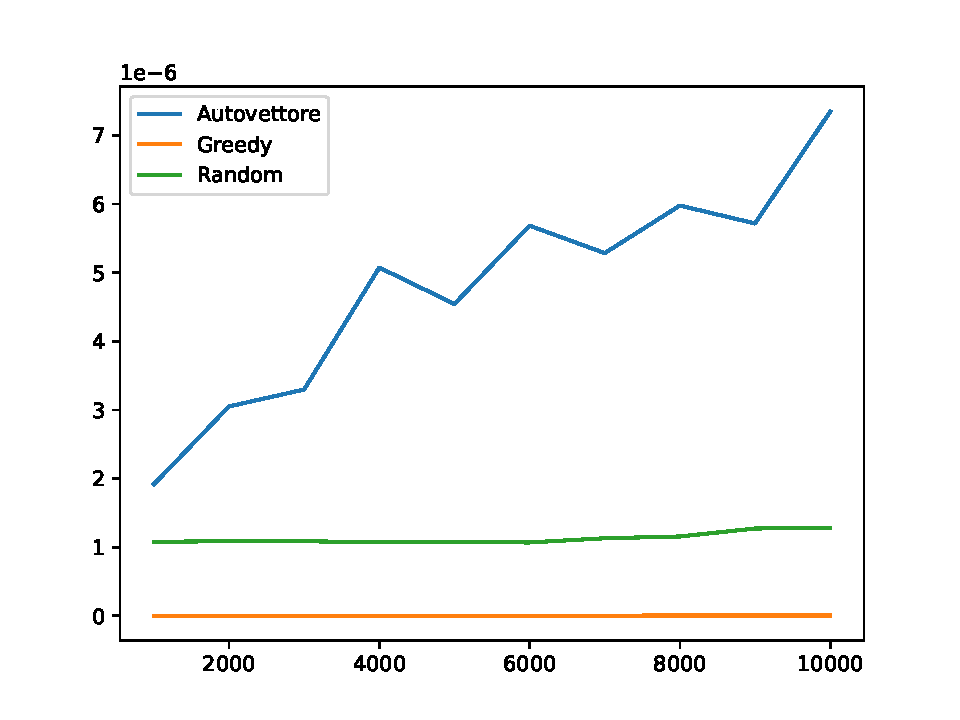
\includegraphics[width=0.7\linewidth]{complexity_plot.pdf}
\end{figure}

\end{document}
